\documentclass[]{article}
\usepackage{lmodern}
\usepackage{amssymb,amsmath}
\usepackage{ifxetex,ifluatex}
\usepackage{fixltx2e} % provides \textsubscript
\ifnum 0\ifxetex 1\fi\ifluatex 1\fi=0 % if pdftex
  \usepackage[T1]{fontenc}
  \usepackage[utf8]{inputenc}
\else % if luatex or xelatex
  \ifxetex
    \usepackage{mathspec}
  \else
    \usepackage{fontspec}
  \fi
  \defaultfontfeatures{Ligatures=TeX,Scale=MatchLowercase}
\fi
% use upquote if available, for straight quotes in verbatim environments
\IfFileExists{upquote.sty}{\usepackage{upquote}}{}
% use microtype if available
\IfFileExists{microtype.sty}{%
\usepackage{microtype}
\UseMicrotypeSet[protrusion]{basicmath} % disable protrusion for tt fonts
}{}
\usepackage[margin=1in]{geometry}
\usepackage{hyperref}
\hypersetup{unicode=true,
            pdfborder={0 0 0},
            breaklinks=true}
\urlstyle{same}  % don't use monospace font for urls
\usepackage{graphicx,grffile}
\makeatletter
\def\maxwidth{\ifdim\Gin@nat@width>\linewidth\linewidth\else\Gin@nat@width\fi}
\def\maxheight{\ifdim\Gin@nat@height>\textheight\textheight\else\Gin@nat@height\fi}
\makeatother
% Scale images if necessary, so that they will not overflow the page
% margins by default, and it is still possible to overwrite the defaults
% using explicit options in \includegraphics[width, height, ...]{}
\setkeys{Gin}{width=\maxwidth,height=\maxheight,keepaspectratio}
\IfFileExists{parskip.sty}{%
\usepackage{parskip}
}{% else
\setlength{\parindent}{0pt}
\setlength{\parskip}{6pt plus 2pt minus 1pt}
}
\setlength{\emergencystretch}{3em}  % prevent overfull lines
\providecommand{\tightlist}{%
  \setlength{\itemsep}{0pt}\setlength{\parskip}{0pt}}
\setcounter{secnumdepth}{5}
% Redefines (sub)paragraphs to behave more like sections
\ifx\paragraph\undefined\else
\let\oldparagraph\paragraph
\renewcommand{\paragraph}[1]{\oldparagraph{#1}\mbox{}}
\fi
\ifx\subparagraph\undefined\else
\let\oldsubparagraph\subparagraph
\renewcommand{\subparagraph}[1]{\oldsubparagraph{#1}\mbox{}}
\fi

%%% Use protect on footnotes to avoid problems with footnotes in titles
\let\rmarkdownfootnote\footnote%
\def\footnote{\protect\rmarkdownfootnote}

%%% Change title format to be more compact
\usepackage{titling}

% Create subtitle command for use in maketitle
\newcommand{\subtitle}[1]{
  \posttitle{
    \begin{center}\large#1\end{center}
    }
}

\setlength{\droptitle}{-2em}
  \title{}
  \pretitle{\vspace{\droptitle}}
  \posttitle{}
  \author{}
  \preauthor{}\postauthor{}
  \date{}
  \predate{}\postdate{}

\geometry{paper=a4paper, margin=2.2cm}
\usepackage[defaultlines=10,all]{nowidow}
\usepackage{float}

\usepackage{fancyhdr}
\pagestyle{fancy}
\lhead{\rightmark}
\rhead{Projet de transcription de musique}

\makeatletter
\renewcommand{\fps@figure}{H}
\makeatother

\AtBeginDocument{\let\maketitle\relax}

%%%%%%%%%%%%%%%% COVER

\makeatletter
\setlength{\parindent}{0cm}
\setlength{\parskip}{1ex plus 0.5ex minus 0.2ex}
\newcommand{\hsp}{\hspace{20pt}}
\newcommand{\HRule}{\rule{\linewidth}{0.5mm}}
\makeatother

\begin{document}

\begin{titlepage}
  \begin{sffamily}
  \begin{center}
	
\includegraphics[width=0.8\textwidth]{img/INSA_logo}\\[2cm]

    \textsc{\huge Département Génie Mathématique}\\[0.7cm]
    %\textsc{\Large }\\[1.5cm]

    % Title
    \HRule \\[0.4cm]
    {\huge \bfseries Projet de transcription de musique \\[0.4cm]}
    \HRule \\[1cm]
	\textsc{\huge rapport d'avancement du projet semestriel}\\[0.7cm]

    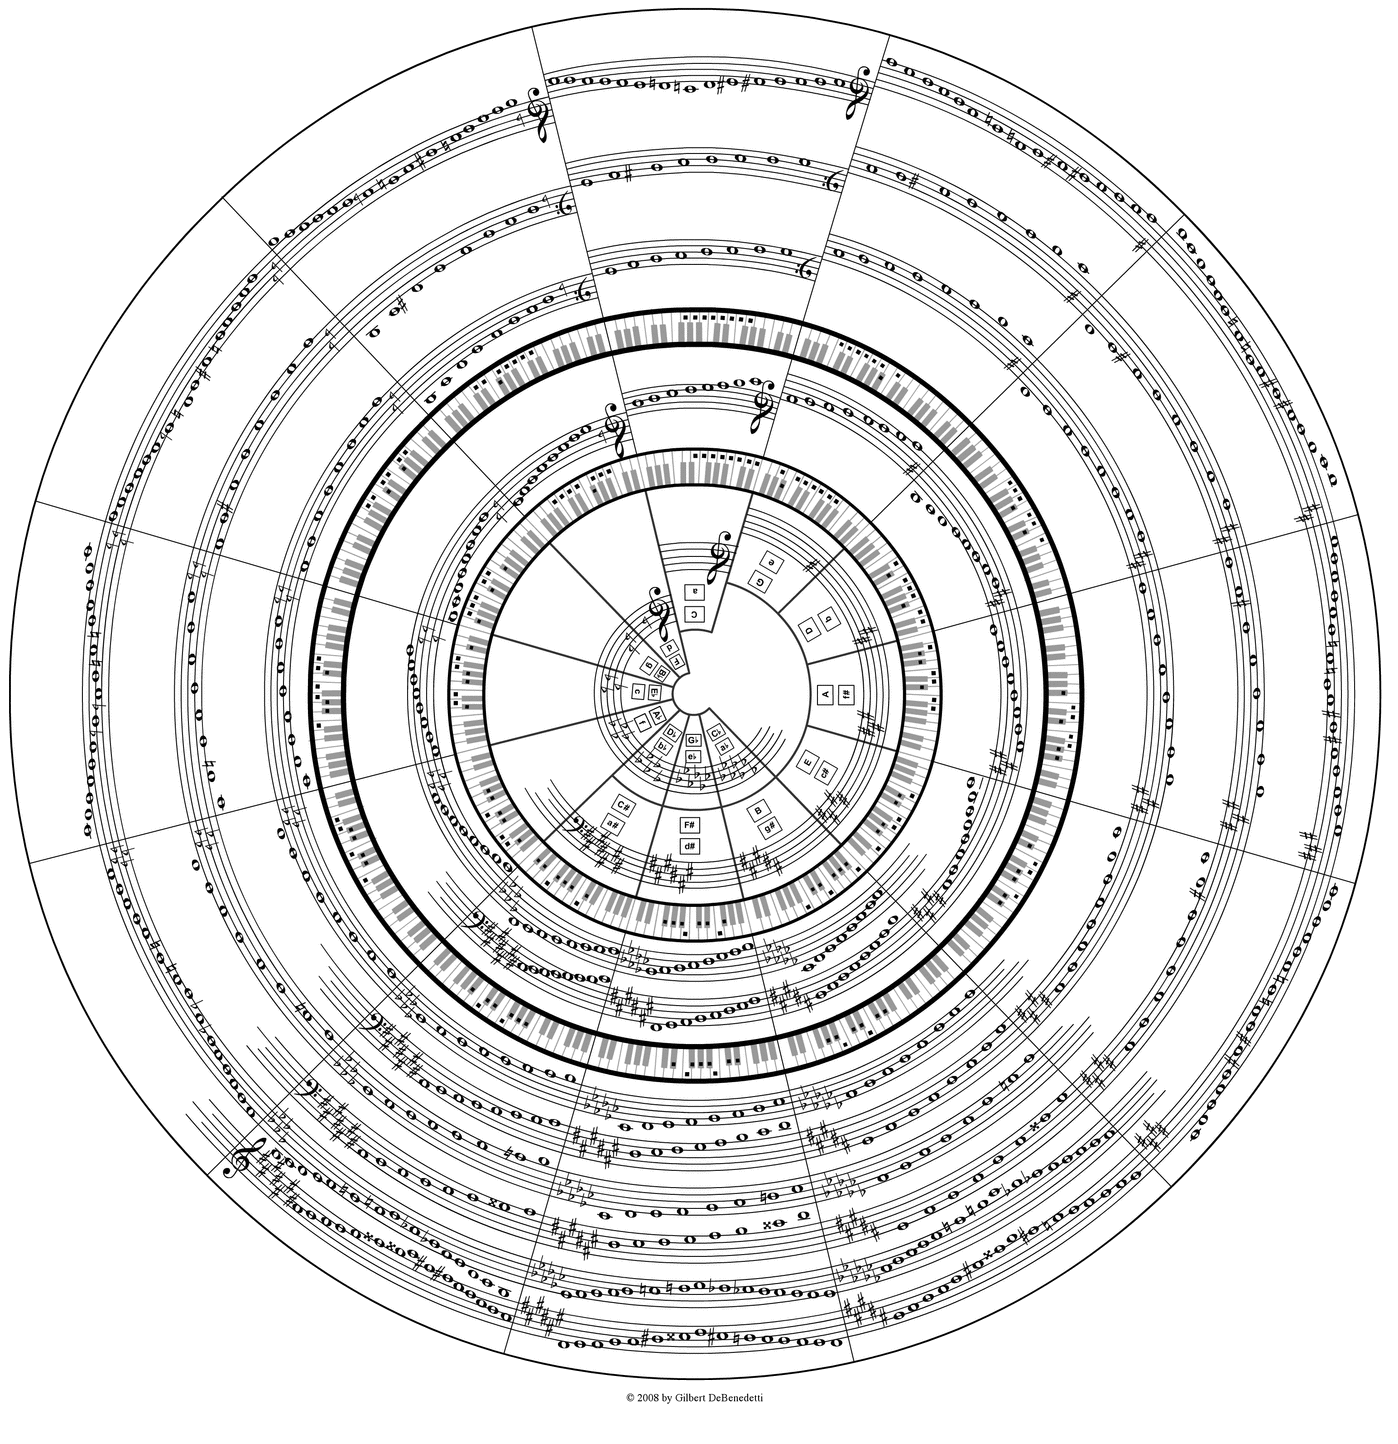
\includegraphics[width=.6\textwidth]{img/cover_img.png}~\\[1cm]

    % Author and supervisor
    \begin{minipage}{0.4\textwidth}
		\Large\raggedright
        Rand ASSWAD\\
		Ergi DIBRA\\
		Yuge SUN
    \end{minipage}
    \begin{minipage}{0.4\textwidth}
		\Large\raggedleft
		\emph{A l'attention de :}\\
		Mme. Natalie FORTIER
    \end{minipage}

	\vfill
    % Bottom of the page
    %{\large 5 mai 2018}
  \end{center}
  \end{sffamily}
\end{titlepage}

{
\setcounter{tocdepth}{2}
\tableofcontents
}
\pagebreak

\hypertarget{introduction}{%
\section{Introduction}\label{introduction}}

La reconnaissance automatique de la musique est une partie essentielle
des logiciels de traitment de musique.

Les résultats d'une reconnaissance automatique sont utilisable dans des
applications nombreuses. Beaucoup d'efforts sont

Nous nous sommes intéressés par la transcription de la musique. Ainsi,
nous avons choisi de travailler sur ce sujet dans le cadre du projet
semestriel. Pendant le développement de ce projet, nous avons dû
apprendre les bases du traitement de signaux sonores et par la suite
étudier les recherches effectuées sur les méthodes de reconnaissance.

Dans ce rapport, nous présentons une analyse de signaux sonores et une
méthode simple de reconnaissance de musique monophones.

\hypertarget{signaux-sonores}{%
\section{Signaux sonores}\label{signaux-sonores}}

\hypertarget{son-harmonique}{%
\subsection{Son harmonique}\label{son-harmonique}}

Le son d'un résonateur acoustique comme une chorde ou une colonne d'air
est une onde stationnaire. On dit que tel son évoque un \textbf{pitch
défini}. Dans le cas des instrument de percussion, le son présente une
\emph{inharmonicité}. On dit que tel son évoque un \textbf{pitch
indéfini}. Dans ce projet on ne s'intéressera qu'au sons harmoniques de
pitch défini.

Un signal sonore de pitch défini, est une série harmonique de sons purs,
représenté par des ondes sinusoïdales dont les fréquences sont des
multiples \textbf{entiers} d'une fréquence dîte la \textbf{fondamentale}
(où le \textbf{pitch}) notée \(f_0\).

\[ x(t) = \sum\limits_{k\in\mathbb{N}} A_k\cdot\cos(2\pi k f_0 t) \] où
\(A_k\) est l'amplitude de la k\textsuperscript{ème} harmonique.

On cherche donc à indentifier \emph{f\_0} dans un signal harmonique
donnée.

\hypertarget{la-transformee-de-fourier-et-ses-variantes}{%
\subsection{La transformée de Fourier et ses
variantes}\label{la-transformee-de-fourier-et-ses-variantes}}

La transformée de Fourier permet d'identifier la fréquence d'une
fonction périodique.
\[\hat{x}(f) = \int\limits_{-\infty}^{\infty} x(t)\cdot e^{-2\pi j ft}\mathrm{d}t\]
Le pic de \(\hat{x}(f)\) correspond à la fréquence du signal \(x(t)\).
Comme la transformée de Fourier est linéaire, la transformée d'un signal
harmonique produit plusieurs pics.

\begin{figure}
\centering
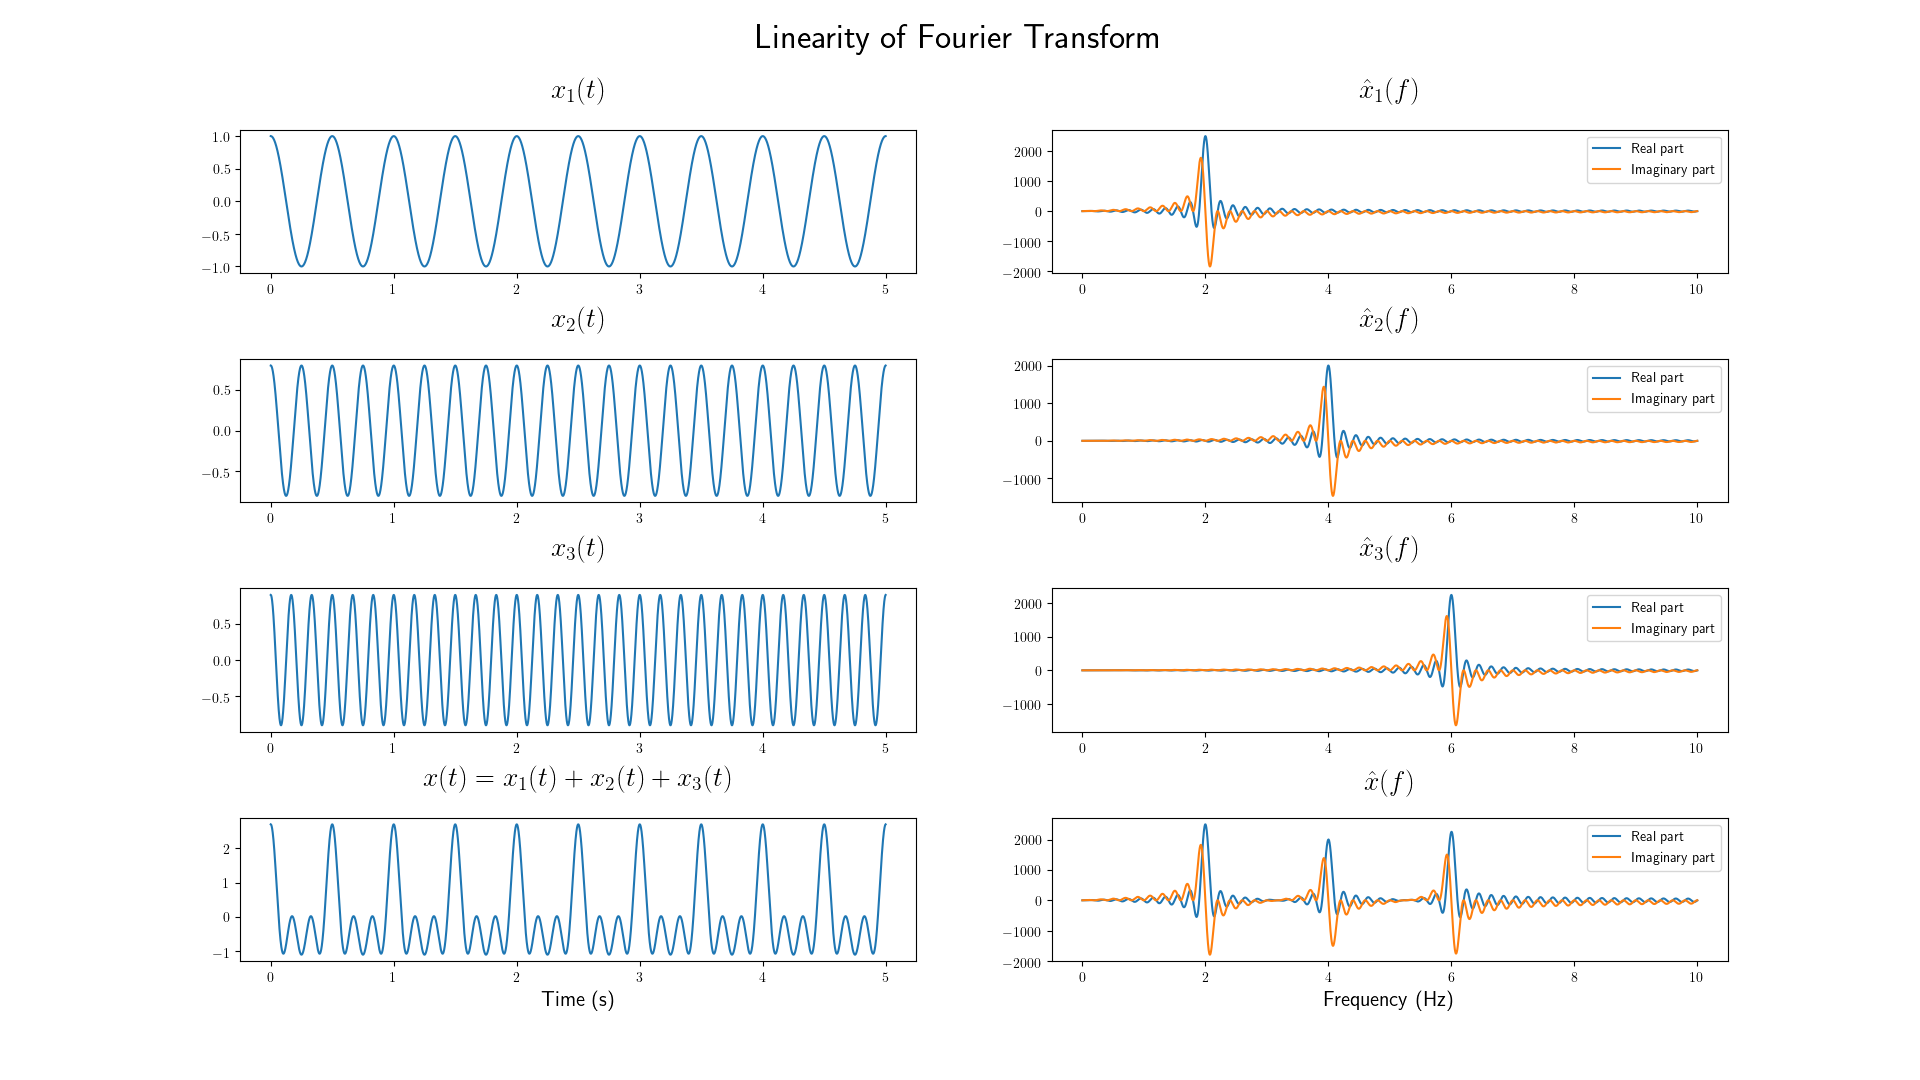
\includegraphics{plot/fourier_linearity.png}
\caption{Linéarité de la transformée de Fourier}
\end{figure}

\hypertarget{la-transformee-de-fourier-a-court-terme}{%
\subsection{La transformée de Fourier à court
terme}\label{la-transformee-de-fourier-a-court-terme}}

Grâce à la transformée de Fourier et sa linéarité on peut obtenir les
fréquences d'un signal harmonique. Or, en pratique, un signal sonore
change souvent de fréquences, on voudrait donc obtenir la transformée de
Fourier en fonction du temps \textbf{et} de la fréquence, la transformée
de Fourier à court terme (anglais: \emph{Short-Time Fourier Transform})
souvent dîte \textbf{STFT} permet d'obtenir tel fonction.

La STFT se calcule à l'aide d'une \textbf{fonction de fenêtrage} \(w\),
qui est une fonction à support compact. En effet, la STFT est la
transformée de Fourier d'une fonction pondérée avec une fenêtre \(w\) de
support compact suffisamment petit. Le principe de cette transformée est
analogue au produit de convolution.

\[X(t, f) = \int\limits_{-\infty}^{\infty} x(\tau)\cdot w(\tau-t)\cdot e^{-2\pi j f\tau} \mathrm{d}\tau \]

\hypertarget{la-transformee-de-fourier-discrete}{%
\subsection{La transformée de Fourier
discrète}\label{la-transformee-de-fourier-discrete}}

Dans ce projet, on voudrais analyser un son enregistré, on étudie donc
le signal sur un intervalle fermé en temps discret.

Soit \(N\) le nombre d'échantillons pris sur l'intervalle
\([0,t_{\text{max}}[\). On introduit la fréquence d'échantillonnage
\(f_s\) dîte en anglais \emph{sample rate} ou \emph{sampling frequency}.
On a donc \(t_n = \frac{n}{f_s}\) pour \(n\in\{0,1,\dots,N-1\}\).

\begin{align}
\hat{x}(f) &= \int\limits_{0}^{t_{\text{max}}} x(t)\cdot e^{-2\pi j ft}\mathrm{d}t \\
    &= \lim\limits{f_s\rightarrow\infty} \sum\limits_{n=0}^{N-1} x(t_n)\cdot e^{-2\pi j ft_n}\\
    &= \lim\limits{f_s\rightarrow\infty} \sum\limits_{n=0}^{N-1} x(t_n)\cdot e^{-2\pi j f \frac{n}{f_s}}
\end{align}

On note \(x[n] = x(t_n)\) on a donc
\[ \hat{x}(f) = \sum\limits_{n=0}^{N-1} x[n]\cdot e^{-2\pi j f \frac{n}{f_s}}\]

On peut également discrétiser la fréquence en définissant
\(X[k]=\hat{x}(f)\).
\[ X[k] = \sum\limits_{n=0}^{N-1} x[n]\cdot e^{-2\pi j k \frac{n}{f_s}}\]

De même, STFT se discrétise:
\[X[n, k] = \sum\limits_{n=0}^{N-1} x[m]\cdot w[m-n]\cdot e^{-2\pi j k \frac{m}{f_s}}\]

Cette partie est une sur-simplification du théroème d'échantillonnage de
\textbf{Nyquist-Shannon}.

\hypertarget{fenetrage}{%
\subsection{Fenêtrage}\label{fenetrage}}

Il existe une infinité de fenêtres à utiliser dans les calculs. La plus
simple est la fonction rectangulaire, mais nous avons utilisé dans
l'intégralité du projet la fonction \textbf{Hann}.

Le choix de la fonction est basé sur un le phénomène du
\textbf{aliasing} qui rend les signaux indisntinguables lors de
l'échantillonnage. En effet, la fenêtre Hann cause peu de
\emph{aliasing} d'où notre choix.

\[w[n] = \sin^2\left(\frac{\pi n}{N -1}\right) =\frac{1}{2}\left(1-\cos\left(\frac{2\pi n}{N -1}\right)\right)\]
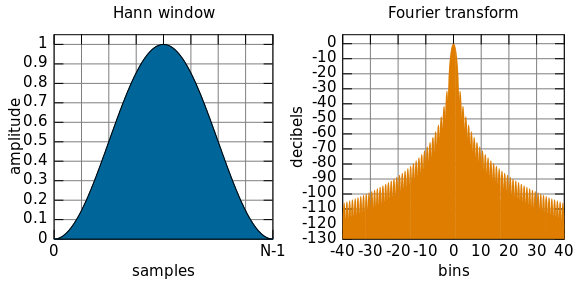
\includegraphics{img/Hann.png}

\hypertarget{pitch}{%
\section{Pitch}\label{pitch}}

Ils existent plusieurs algorithmes de détection de fréqences
fondamentales, il y'en a deux types : applications sur le domaine
temporel et sur le domaine fréquenciel. Les applications sur le domaine
fréquenciel calculent les fréquences à partir de la transformée de
Fourier du signal, où les méthodes du domaine temporel les calcules à
partir du signal sans passer par la transformée de Fourier.

Chaque type présente des avantages et des inconvénients. Nous avons
décidé d'implémenter une de chaque type:

\hypertarget{yin}{%
\subsection{YIN}\label{yin}}

L'algorithme de YIN \emph{(Kawahara et de Cheveigné, 2002)} est une
méthode robuste pour la reconnaissance du pitch, il s'agit d'un modèle
temporel. Son principe est la séléction de fréquences candidats parmi
toutes les fréquences détéctés sur l'intervalle de fenêtrage.

La méthode propose que l'expression \(x(t)-x(t+\tau)\) atteint son
minimum quand \(\tau\) est égale à la période du signal (i.e.
\(\frac{1}{f_0}\)). En diffinissant la fonction de différence à
l'instant \(t\) fixé:
\[ d_t(\tau) = \int\limits_{t}^{t+T_w} \left(x(t)-x(t+\tau)\right)^2 \mathrm{d}t \]
où \(T_w\) est la taille de la fenêtre \(w\), on appelle \(\tau\) le
\emph{retard} (anglais: \emph{lag}).

Soit en temps discret:
\[ d_n[m] = \sum\limits_{i=n+1}^{n+N_w} \left(x[n]-x[n+m]\right)^2 \]

Par la suite, on calcule la fonction de la moyenne cumulative définie
par: \[d_t'(\tau) = \begin{cases}
1 &\text{si} \tau = 0\\
d_t(\tau) / \frac{1}{\tau}\int\limits_{0}^{\tau}d_t(u)\mathrm{d}u &\text{sinon}
\end{cases}\] Soit en temps discret: \[d_n'[m] = \begin{cases}
1 &\text{si} m = 0\\
d_n[m] / \frac{1}{m}\sum\limits_{i=0}^{m}d_t[i] &\text{sinon}
\end{cases}\]

Les candidats sont les minimums locaux de \(d_n'\).

\hypertarget{yin-spectrale}{%
\subsection{YIN spectrale}\label{yin-spectrale}}

L'algorithme de YIN spectrale \emph{(Paul Brossier, 2006)} est une
méthode qui utilise la même logique de l'algorithme de YIN et l'applique
sur la STFT.

La fonction de différence est définie par: \[ \hat{d}_n[m] = \frac{2}{N}
\sum\limits_{k=0}^{\frac{N}{2}+1}
\left\lvert\left( 1-e^{2\pi jkm/N} \right)   X[n,k]  \right\rvert^2 \]

La fonction de la moyenne cumulative se calcule de façon analogue à
l'algorithme de YIN. L'algorithme cherche le minimum globale de cette
dernière.

\hypertarget{segmentation-temporelle}{%
\section{Segmentation temporelle}\label{segmentation-temporelle}}

L'étape fondamentale dans la reconnaissance du son est la segmentation
temporelle. Il s'agit de trouver les frontières des objets sonores,
c'est-à-dire:

\begin{itemize}
\tightlist
\item
  Le début de la note -- dît \textbf{\emph{onset}}.
\item
  La fin de la note -- dît \textbf{\emph{offset}}.
\end{itemize}

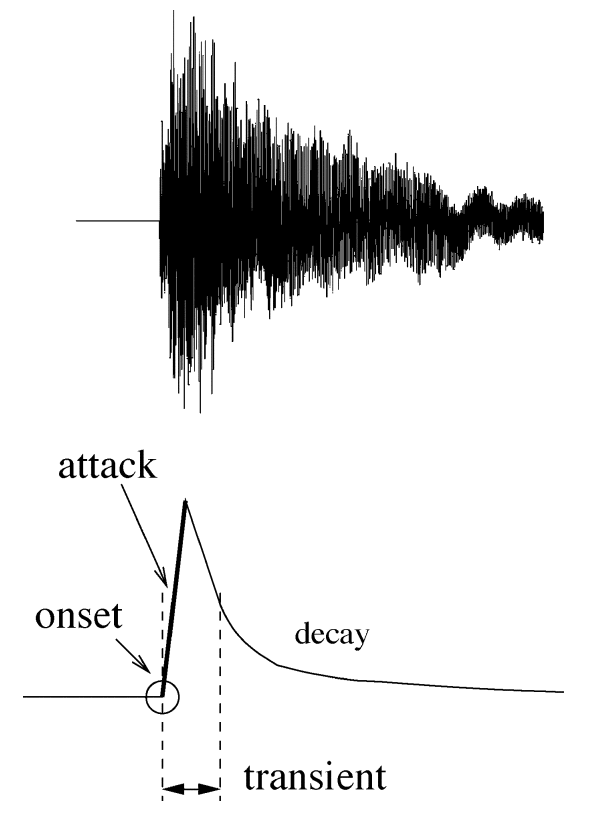
\includegraphics[width=0.5\textwidth,height=\textheight]{img/onset.png}

Attack, transient, decay, onset IEEE TRANSACTIONS ON SPEECH AND AUDIO
PROCESSING, VOL. 13, NO. 5, SEPTEMBER 2005

Cette étape dépend fortement sur le type du son produit; les instrument
à chordes pincées (guitare, piano, oud, etc.) ont un profile différent
de celui des instruments à cordes frottées (la famille du violon) ou de
celle des instruments à vent.

Dans cette partie on expliquera les méthodes implémentés pour la
reconnaissance du \textbf{onset}.

\hypertarget{methode}{%
\subsection{Méthode}\label{methode}}

La lecture scientifique indique une méthode rigoureuse qu'on a
simplifier pour obtenir des résultats rapide.

Il s'agit de définir une fonction qui permet de quantifier la
perturbation du signal à un moment donné, cette fonction est souvent
appellée \textbf{Onset Detection Function} ou \textbf{Onset Strength
Signal}, dans ce projet on fera référence à cette dernière par
\textbf{Onset Detection Function} ou \textbf{\emph{ODF}}.

Théoriquement, les maximums locaux de l'ODF sont les onsets du signal,
mais en pratique il s'agit d'un sous-ensemble de ces points. En effet,
l'ODF est souvent très sensible et détectera la moindre des
perturbations.

Ce problème pourra être résolu en définissant un seuil au dessous duquel
aucun onset est considéré. Ils existent plusieurs méthodes pour définir
tel seuil.

Soit un seuil fixe, ce qui minimise le coût des calculs au prix de la
qualité des résultats. Soit de calculer un seuil variable, il s'agit de
lisser la fonction ODF par des méthodes classiques comme la moyenne
mobile.

La méthode consiste donc en trois étapes: 1. Calcul de l'\textbf{Onset
Detection Function}. 2. \textbf{Thresholding}: calcul du seuil. 3.
\textbf{Peak-picking}: la selection des onsets.

\hypertarget{onset-detection-function-odf}{%
\subsection{Onset Detection Function
(ODF)}\label{onset-detection-function-odf}}

Ils existent plusieurs fonction de détéction d'onsets, on expliquera
quelques unes qui se basent sur la STFT.

\hypertarget{high-frequency-content-hfc}{%
\subsubsection{High Frequency Content
(HFC)}\label{high-frequency-content-hfc}}

Il s'agit de priviligier les fréquences élevées dans un signal:
\[ HFC[n] = \sum\limits_{k=1}^{N}k\cdot\left\lvert X[n,k]\right\rvert^2 \]

\hypertarget{phase-deviation-phi}{%
\subsubsection{Phase Deviation (Phi)}\label{phase-deviation-phi}}

Il s'agit de calculer les différences de phases en dérivant l'argument
complex de la STFT, on note \$\varphi(t, f) = \mathrm{arg}(X(t, f)) \$.
\[\hat{\varphi}(t, f) = \mathrm{princarg}
\left( \frac{\partial^2 \varphi}{\partial t^2}(t, f)  \right) \] où
\[ \mathrm{princarg}(\theta) = \pi + ((\theta + \pi) mod (-2\pi)) \]
donc la ODS de phase se calcule par la formule:
\[ \Phi[n] = \sum\limits_{k=0}^{N}\left\lvert \hat{\varphi}[n, k] \right\rvert \]

Dans notre implémentation, nous avons approximé la dérivée partielle
seconde de la phase par un schéma de Taylor d'ordre 2.

\hypertarget{complex-distance}{%
\subsubsection{Complex Distance}\label{complex-distance}}

Cette méthode permet de qualifier les changements spectraux du signal
ainsi que les changements en phase. Il s'agit de calculer une prédiction
du spectre du signal, et puis le comparer par sa valeur. On reprend la
fonction calculée en \(\hat{varphi}(t, f)\) de la méthode précédante. On
définit la prédiction :
\[ \hat{X}[n, k] = \left\lvert X[n, k] \right\rvert \cdot e^{j\hat{\varphi}[n, k]} \]

Donc la distance complexe se calcule:
\[ DC[n] = \sum\limits_{k=0}^{N} \left\lvert  \hat{X}[n, k] - X[n, k] \right\rvert ^2 \]

\hypertarget{thresholding}{%
\subsection{Thresholding}\label{thresholding}}

Nous avons décidé de lisser la fonction ODF par une moyenne mobile
echelonnées par la fenêtre Hann, il s'agit du produit de convolution de
l'ODF avec la fonction Hann.


\end{document}
